\documentclass[article,12pt,oneside,a4paper,english,brazil]{abntex2}

\usepackage{lmodern}
\usepackage[T1]{fontenc}
\usepackage[utf8]{inputenc}
\usepackage{indentfirst}
\usepackage{xcolor}
\usepackage{graphicx}
\usepackage{amsmath,amssymb}
\usepackage{booktabs}
\usepackage{tabularx}
\usepackage{tikz}
\usetikzlibrary{arrows.meta,positioning}
\usepackage[brazilian,hyperpageref]{backref}
\usepackage[alf]{abntex2cite}

% Trechos em vermelho devem ser conferidos/ajustados pelo autor antes da entrega
\newcommand{\pendente}[1]{\textcolor{red}{#1}}
\newcommand{\NRODADAS}{\pendente{N}}
\newcommand{\TEMPODIG}{\pendente{--}}
\newcommand{\TEMPOOCR}{\pendente{--}}
\newcommand{\RESULTADOSDESEMPENHO}{\pendente{[desempenho]}}
\newcommand{\CONCLUSAODESEMPENHO}{\pendente{[conclusão desempenho]}}

\setlrmarginsandblock{3cm}{2cm}{*}
\setulmarginsandblock{3cm}{2cm}{*}
\checkandfixthelayout
\setlength{\parindent}{1.25cm}
\setlength{\parskip}{0.2cm}
\OnehalfSpacing

\renewcommand{\ABNTEXchapterfont}{\rmfamily\bfseries}
\renewcommand{\ABNTEXsectionfont}{\rmfamily\bfseries}
\renewcommand{\ABNTEXsectionfontsize}{\normalsize}
\renewcommand{\ABNTEXsectionupperifneeded}{\MakeUppercase}
\renewcommand{\ABNTEXsubsectionfont}{\rmfamily\bfseries}
\renewcommand{\ABNTEXsubsectionfontsize}{\normalsize}
\renewcommand{\ABNTEXsubsubsectionfont}{\rmfamily\bfseries}
\renewcommand{\ABNTEXsubsubsectionfontsize}{\normalsize}

\renewcommand{\backrefpagesname}{}
\renewcommand{\backref}{}

\begin{document}

\selectlanguage{brazil}
\frenchspacing

% ---------------------------------------------------------------------------
% Título e autores
% ---------------------------------------------------------------------------
\begin{center}
\textbf{VALIDAÇÃO AUTOMATIZADA DE CARNÊS: um sistema baseado em reconhecimento óptico
de caracteres e extração orientada por \textit{layout} para a conferência de documentos
tributários municipais}

\vspace{0.4cm}
\textit{Automated Validation of Tax Payment Booklets: an optical character recognition
and layout-driven extraction system for auditing municipal tax documents}

\vspace{0.6cm}
Normando Nascimento Oliveira Meira\footnote{Graduando, FATEC Ribeirão Preto -- SP.
E-mail: \pendente{normando.meira@aluno.cps.sp.gov.br}}

Lucas Baggio Figueira\footnote{\pendente{Mestre}, FATEC Ribeirão Preto -- SP.
E-mail: \pendente{lucas.figueira@cps.sp.gov.br}}
\end{center}

% ---------------------------------------------------------------------------
% Resumo
% ---------------------------------------------------------------------------
\vspace{0.4cm}
\noindent\textbf{RESUMO}\par
\noindent Este trabalho apresenta o SMARsvd, um sistema de validação automatizada de carnês
e guias de tributos municipais emitidos em PDF, que combina extração de texto
orientada por \textit{layout}, reconhecimento óptico de caracteres (\textit{Optical
Character Recognition} -- OCR) e consultas de somente leitura ao banco de dados
tributário para identificar divergências antes da distribuição dos documentos aos
contribuintes. O sistema permite que o usuário descreva, uma única vez e sem
programação, onde cada informação se encontra no documento; a partir disso,
segmenta lotes com milhares de páginas em documentos individuais, extrai os campos
priorizando a camada de texto digital e recorre ao OCR (Tesseract) apenas nas regiões
sem texto, interpreta os valores conforme o tipo de dado esperado e os compara com o
cadastro oficial. A avaliação foi conduzida sobre lotes reais de carnês de
parcelamento de um município paulista, com 188 e 11.584 páginas, em dois cenários:
extração digital e extração exclusivamente por OCR, simulando documentos digitalizados.
No cenário digital, todos os documentos foram segmentados e todos os campos presentes
foram extraídos corretamente. No cenário de OCR, a segmentação manteve 100\% de acerto
e 92,9\% dos valores foram recuperados; os 7,1\% restantes foram sinalizados como
ausentes ou inválidos, sem nenhum caso de valor incorreto aceito silenciosamente.
Os resultados indicam que a estratégia híbrida, associada à validação por tipo de dado,
torna o OCR uma alternativa segura para a conferência automatizada de documentos
fiscais.

\noindent\textbf{Palavras-chave}: reconhecimento óptico de caracteres; extração de dados;
validação de documentos; administração tributária.

\begin{otherlanguage*}{english}
\noindent\textbf{ABSTRACT}\par
\noindent This paper presents SMARsvd, an automated validation system for municipal tax
payment booklets and bills issued as PDF files. It combines layout-driven text
extraction, optical character recognition (OCR) and read-only queries to the tax
database in order to detect inconsistencies before documents are delivered to
taxpayers. Users describe, only once and without programming, where each piece of
information is located on the document; the system then splits batches with thousands
of pages into individual documents, extracts fields prioritizing the digital text
layer and falls back to OCR (Tesseract) only for regions without text, parses values
according to the expected data type and compares them with the official records. The
evaluation used real batches of installment booklets from a municipality in São Paulo
state, with 188 and 11,584 pages, under two scenarios: digital extraction and OCR-only
extraction, simulating scanned documents. In the digital scenario, every document was
correctly segmented and every existing field was correctly extracted. In the OCR
scenario, segmentation remained 100\% accurate and 92.9\% of the values were recovered;
the remaining 7.1\% were flagged as missing or invalid, with no incorrect value
silently accepted. Results suggest that the hybrid strategy, combined with data-type
validation, makes OCR a safe alternative for automated auditing of tax documents.

\noindent\textbf{Keywords}: optical character recognition; data extraction; document
validation; tax administration.
\end{otherlanguage*}

% ---------------------------------------------------------------------------
\section{Introdução}
% ---------------------------------------------------------------------------

A Constituição Federal atribui aos municípios a competência para instituir impostos
como o IPTU, o ISS e o ITBI \cite{brasil1988}. A cobrança desses tributos, bem como
de taxas e parcelamentos de débitos, materializa-se em carnês e guias que são gerados
anualmente em grande volume, normalmente em um único arquivo PDF com centenas ou
milhares de páginas, posteriormente encaminhado à gráfica ou disponibilizado aos
contribuintes. Qualquer inconsistência nesses documentos -- um valor, uma inscrição
imobiliária, um CPF ou uma data de vencimento divergente do cadastro -- tende a ser
percebida somente após a entrega, gerando retrabalho, atendimento adicional, desgaste
institucional e risco à arrecadação.

A conferência desses arquivos costuma ser manual e amostral: um servidor abre algumas
páginas e compara visualmente os dados impressos com os registros do sistema
tributário. Esse procedimento é lento, cansativo e sujeito a falhas, e sua cobertura
diminui justamente quando o volume de documentos aumenta. A transformação digital do
setor público brasileiro tem buscado substituir processos dessa natureza por soluções
automatizadas e orientadas a dados \cite{oecd2018}, o que motiva o uso de técnicas de
extração automática de informações de documentos.

O reconhecimento óptico de caracteres (\textit{Optical Character Recognition} -- OCR) é a
tecnologia que converte imagens de texto em texto processável por máquina
\cite{islam2017,memon2020}. Motores de código aberto como o Tesseract
\cite{smith2007} tornaram viável sua aplicação local, sem envio de dados a serviços
externos -- aspecto relevante quando os documentos contêm dados pessoais protegidos pela
Lei Geral de Proteção de Dados \cite{brasil2018lgpd}. Entretanto, o OCR isoladamente
não resolve o problema: é preciso saber \emph{onde} está cada informação, separar
documentos dentro de um lote, isolar o valor de interesse no texto lido e, sobretudo,
confrontá-lo com a fonte oficial de dados.

O presente trabalho propõe e avalia o SMARsvd (Sistema de Validação de Documentos), uma
aplicação web desenvolvida em C\#/.NET e React que automatiza essa conferência. O
sistema adota uma estratégia híbrida de extração -- camada de texto digital do PDF
quando disponível e OCR apenas como alternativa --, orientada por \textit{layouts}
configuráveis pelo próprio usuário, e compara os valores extraídos com os retornados
por consultas SQL de somente leitura ao banco de dados tributário. A principal
contribuição está na integração, em um único fluxo, da segmentação de lotes, da
extração híbrida, da interpretação tipada dos valores e da auditoria contra o cadastro
oficial, acompanhada de uma avaliação empírica com documentos reais.

O restante deste trabalho é organizado da seguinte maneira: a Seção~\ref{sec:revisao}
apresenta a revisão da literatura; o método de pesquisa é descrito na
Seção~\ref{sec:metodo}; a Seção~\ref{sec:modelagem} apresenta a modelagem do sistema
proposto; os experimentos computacionais são descritos na
Seção~\ref{sec:experimentos}; os resultados são apresentados e discutidos na
Seção~\ref{sec:resultados} e, por fim, a Seção~\ref{sec:consideracoes} apresenta as
considerações finais.

% ---------------------------------------------------------------------------
\section{Revisão bibliográfica}\label{sec:revisao}
% ---------------------------------------------------------------------------

Esta seção organiza a literatura em torno de três eixos: o reconhecimento óptico de
caracteres e o motor Tesseract, a extração de informações de documentos estruturados e
os requisitos de segurança e privacidade envolvidos no tratamento de dados fiscais.

O OCR é um problema clássico de reconhecimento de padrões, tradicionalmente dividido nas
etapas de aquisição da imagem, pré-processamento, segmentação, extração de
características, classificação e pós-processamento \cite{islam2017}. Memon et al.
\cite{memon2020}, em revisão sistemática da literatura, destacam que o desempenho dos
sistemas de OCR depende fortemente da qualidade da imagem de entrada e que as etapas de
pré-processamento -- conversão para tons de cinza, ajuste de contraste, redimensionamento
e remoção de ruído -- têm impacto direto na taxa de acerto. A documentação oficial do
Tesseract reforça essa orientação, recomendando imagens com resolução em torno de
300~DPI e altura de caractere suficiente para o reconhecimento
\cite{tessdocqualidade}.

O Tesseract, originalmente desenvolvido pela HP e posteriormente mantido como projeto de
código aberto, é descrito por Smith \cite{smith2007} como um motor que combina análise
de componentes conectados, detecção de linhas e palavras e classificação adaptativa de
caracteres. As versões recentes incorporam redes neurais recorrentes do tipo LSTM e
oferecem modelos treinados para dezenas de idiomas, inclusive o português. Patel, Patel
e Patel \cite{patel2012} compararam o Tesseract a uma ferramenta comercial e obtiveram
acurácia superior com a solução aberta, além da vantagem de custo, o que justifica sua
adoção em aplicações com restrições orçamentárias, como as do setor público.

A extração de informações de documentos vai além do reconhecimento de caracteres,
pois exige localizar e rotular campos específicos. A competição SROIE, dedicada a
recibos digitalizados, formalizou esse problema em três tarefas: localização de texto,
reconhecimento e extração de campos-chave \cite{huang2019sroie}. Abordagens recentes
baseadas em aprendizado profundo, como o LayoutLM \cite{xu2020layoutlm}, que combina
texto e posição espacial em um modelo pré-treinado, e o Donut \cite{kim2022donut}, que
dispensa o OCR ao gerar a saída estruturada diretamente da imagem, alcançam resultados
expressivos em documentos heterogêneos. Contudo, esses modelos exigem grandes volumes de
dados anotados, capacidade computacional significativa e, em muitos casos, execução em
nuvem. Para documentos de \textit{layout} fixo e conhecido, como carnês gerados por um
mesmo sistema emissor, a extração orientada por modelo (\textit{template-based}), em que
as regiões de interesse são definidas previamente, permanece uma alternativa mais
simples, previsível e auditável.

Por fim, a validação automatizada exige consultar o banco de dados tributário, o que
introduz riscos de segurança. A OWASP \cite{owasp} aponta a injeção de SQL como uma das
vulnerabilidades mais críticas em aplicações que montam consultas dinamicamente e
recomenda, entre outras medidas, a validação das instruções e o princípio do menor
privilégio. Analisadores sintáticos oficiais, como o ScriptDom da Microsoft
\cite{microsoftscriptdom}, permitem inspecionar a árvore sintática de instruções
Transact-SQL antes da execução. Somam-se a isso as exigências da LGPD
\cite{brasil2018lgpd} quanto à minimização e à segurança no tratamento de dados
pessoais, o que favorece soluções executadas localmente, sem transferência de
documentos a serviços de terceiros.

Nenhum dos trabalhos analisados aborda, de forma integrada, a segmentação de lotes de
documentos tributários, a extração híbrida (texto digital e OCR) e a conferência
automática contra a base cadastral oficial -- lacuna que o presente trabalho busca
endereçar.

% ---------------------------------------------------------------------------
\section{Método de pesquisa}\label{sec:metodo}
% ---------------------------------------------------------------------------

Esta pesquisa classifica-se como aplicada, de natureza quantitativa, e adota como
abordagem predominante a \textit{Design Science Research} (DSR), voltada à concepção e
avaliação de artefatos que resolvem problemas práticos
\cite{hevner2004,dresch2015}. O artefato desenvolvido é o sistema SMARsvd, concebido
no contexto de uma empresa de desenvolvimento de software para a gestão pública
municipal, a partir da necessidade real de conferir os carnês emitidos para as
prefeituras clientes antes de sua distribuição.

O desenvolvimento seguiu as etapas propostas por \citeonline{dresch2015}:
(i) identificação e conscientização do problema, por meio da observação do processo
manual de conferência; (ii) revisão da literatura sobre OCR, extração de informações de
documentos e segurança no acesso a dados; (iii) projeto e desenvolvimento do artefato;
(iv) avaliação experimental com documentos reais; e (v) explicitação das aprendizagens e
limitações.

O problema tratado é estruturado em dois objetivos complementares. O primeiro consiste
em extrair, de forma automática e sem intervenção manual por documento, as informações
de interesse de lotes de carnês em PDF, independentemente de o arquivo possuir camada
de texto digital ou ser composto apenas por imagens. O segundo consiste em confrontar
cada informação extraída com o valor correspondente no banco de dados tributário,
produzindo um relatório que aponte, documento a documento, as divergências encontradas.

Em ambos os objetivos, o sistema deve ser genérico -- capaz de lidar com diferentes
modelos de carnê sem alteração de código --, seguro -- sem possibilidade de alterar o
banco de dados consultado nem de enviar dados a serviços externos -- e escalável para
lotes com milhares de páginas. A avaliação do artefato é conduzida por meio de
experimentos computacionais que medem a acurácia da segmentação e da extração, a taxa
de erro de caracteres do OCR e o tempo de processamento.

% ---------------------------------------------------------------------------
\section{Modelagem do sistema}\label{sec:modelagem}
% ---------------------------------------------------------------------------

O SMARsvd é composto por uma interface web (React e TypeScript) e por um servidor em
ASP.NET Core (.NET 6) organizado em camadas de domínio, aplicação, infraestrutura e
API, conforme os princípios de arquitetura limpa \cite{martin2017}. O fluxo de
validação, ilustrado na Figura~\ref{fig:fluxo}, é formalizado a seguir.

\begin{figure}[htb]
\centering
\caption{Fluxo de validação do SMARsvd}\label{fig:fluxo}
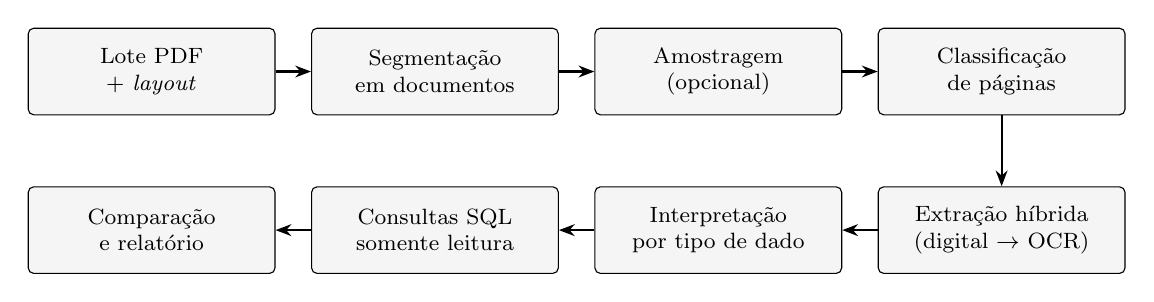
\begin{tikzpicture}[
  node distance=0.35cm and 0.45cm,
  etapa/.style={draw, rounded corners=2pt, align=center, font=\footnotesize,
                minimum height=1.1cm, text width=2.9cm, fill=gray!8},
  seta/.style={-{Stealth[length=2mm]}, thick}
]
\node[etapa] (pdf) {Lote PDF\\+ \textit{layout}};
\node[etapa, right=of pdf] (seg) {Segmentação\\em documentos};
\node[etapa, right=of seg] (amo) {Amostragem\\(opcional)};
\node[etapa, right=of amo] (cla) {Classificação\\de páginas};
\node[etapa, below=0.9cm of cla] (ext) {Extração híbrida\\(digital $\rightarrow$ OCR)};
\node[etapa, left=of ext] (int) {Interpretação\\por tipo de dado};
\node[etapa, left=of int] (sql) {Consultas SQL\\somente leitura};
\node[etapa, left=of sql] (cmp) {Comparação\\e relatório};
\draw[seta] (pdf) -- (seg);
\draw[seta] (seg) -- (amo);
\draw[seta] (amo) -- (cla);
\draw[seta] (cla) -- (ext);
\draw[seta] (ext) -- (int);
\draw[seta] (int) -- (sql);
\draw[seta] (sql) -- (cmp);
\end{tikzpicture}
\legend{Fonte: Autores}
\end{figure}

Seja um lote $A$ com páginas $P = \{1, 2, \ldots, N\}$ e um \textit{layout}
$L = (R, Q)$, em que $R$ é o conjunto de regiões demarcadas pelo usuário sobre um
documento-modelo e $Q$ o conjunto de consultas de validação. Cada região
$r \in R$ é descrita por:

\begin{itemize}
\item $(x_r, y_r, w_r, h_r)$: posição e dimensões do retângulo, em milímetros;
\item $c_r \in \{\mathrm{doc}, \mathrm{pag}, \mathrm{campo}\}$: classificação da região
  como identificador de documento, identificador de página ou campo a ser validado;
\item $e_r$: texto esperado, para regiões identificadoras;
\item $\tau_r \in \{$texto, inteiro, decimal, data, CPF/CNPJ, CEP$\}$: tipo de dado do campo;
\item $a_r, b_r$: textos-âncora anterior e posterior ao valor, opcionais;
\item $g_r$: identificador de página ao qual o campo pertence.
\end{itemize}

A extração do texto de uma região $r$ na página $p$ segue a estratégia híbrida da
Equação~(\ref{eq:hibrida}), em que $T_{\mathrm{dig}}$ é o texto obtido da camada
digital do PDF pela biblioteca PdfPig \cite{pdfpig} e $T_{\mathrm{ocr}}$ é o texto
reconhecido pelo Tesseract \cite{smith2007} a partir da imagem da página:

\begin{equation}\label{eq:hibrida}
T(p, r) =
\begin{cases}
T_{\mathrm{dig}}(p, r), & \text{se } T_{\mathrm{dig}}(p, r) \neq \varnothing \\
T_{\mathrm{ocr}}(p, r), & \text{caso contrário}
\end{cases}
\end{equation}

Na extração digital, as coordenadas em milímetros são convertidas para pontos
tipográficos, e o eixo vertical é invertido, pois a origem do PDF está no canto
inferior esquerdo da página de altura $H$:

\begin{equation}\label{eq:pontos}
x^{\mathrm{pt}} = x_r \cdot \frac{72}{25{,}4}, \qquad
y^{\mathrm{pt}}_{\mathrm{topo}} = H - y_r \cdot \frac{72}{25{,}4}
\end{equation}

Uma palavra é atribuída à região quando há sobreposição horizontal e quando seu
centro vertical está contido no retângulo ou pelo menos 50\% de sua altura se sobrepõe
a ele; as palavras selecionadas são então ordenadas por linha e por posição horizontal.
No caminho de OCR, a página é renderizada a aproximadamente 300~DPI
\cite{tessdocqualidade} e a região é recortada com base na escala
$s = W^{\mathrm{px}} / W^{\mathrm{mm}}$ (cerca de 11,81 px/mm). O recorte é
pré-processado com conversão para tons de cinza, ampliação bicúbica de duas vezes,
aumento de contraste e nitidez gaussiana, e submetido ao Tesseract com o modelo de
língua portuguesa, primeiro no modo de bloco único e, se nada for reconhecido, no modo
de linha única.

A segmentação do lote em documentos utiliza a região identificadora de documento
$r_d$. Sendo $\eta(\cdot)$ uma função de normalização que remove acentos e espaços
excedentes, o conjunto de páginas iniciais é dado pela Equação~(\ref{eq:inicios}), e o
documento $D_k$ corresponde ao intervalo da Equação~(\ref{eq:documento}):

\begin{equation}\label{eq:inicios}
I = \{\, p \in P : \eta(e_{r_d}) \subseteq \eta(T(p, r_d)) \,\} = \{i_1 < i_2 < \cdots < i_K\}
\end{equation}

\begin{equation}\label{eq:documento}
D_k = [\, i_k,\; i_{k+1} - 1 \,], \qquad k = 1, \ldots, K, \quad i_{K+1} = N + 1
\end{equation}

Quando a validação por amostragem é escolhida com percentual $\alpha$, são sorteados
aleatoriamente $n$ documentos, conforme a Equação~(\ref{eq:amostra}):

\begin{equation}\label{eq:amostra}
n = \left\lceil K \cdot \frac{\alpha}{100} \right\rceil
\end{equation}

Para cada campo $r$ de um documento $D_k$, o valor extraído é obtido pela
Equação~(\ref{eq:valor}), em que $\sigma_{a_r, b_r}$ descarta o texto anterior à âncora
$a_r$ e posterior à âncora $b_r$, e $\varphi_{\tau_r}$ aplica uma expressão regular
correspondente ao tipo de dado, retornando o primeiro trecho compatível:

\begin{equation}\label{eq:valor}
v_{k,r} = \varphi_{\tau_r}\!\left(\sigma_{a_r, b_r}\big(T(p, r)\big)\right), \qquad p \in D_k
\end{equation}

Cada valor recebe uma situação: \emph{válido}, quando interpretado com sucesso;
\emph{ausente}, quando a região está vazia ou a âncora não é localizada; ou
\emph{inválido}, quando há texto, mas nenhum trecho compatível com o formato esperado.
Valores inválidos impedem a execução das consultas que dependem deles, evitando
comparações baseadas em leituras incorretas.

Cada consulta $q \in Q$ é uma instrução \texttt{SELECT} escrita pelo usuário com
parâmetros no formato \texttt{\$Campo}. Para cada documento, os parâmetros são
substituídos pelos valores extraídos, formatados segundo seu tipo, e as consultas são
executadas no banco de dados tributário. Por fim, cada regra de validação $j$
associa uma coluna retornada $u_j$ a um campo $r_j$ do documento, e a conferência é
realizada conforme as Equações~(\ref{eq:comparacao}) e (\ref{eq:documentovalido}):

\begin{equation}\label{eq:comparacao}
\delta_{k,j} =
\begin{cases}
1, & \text{se } \mathrm{maiúsc}(v_{k,r_j}) = \mathrm{maiúsc}(u_{k,j}) \\
0, & \text{caso contrário}
\end{cases}
\end{equation}

\begin{equation}\label{eq:documentovalido}
\mathrm{válido}(D_k) = \prod_{j} \delta_{k,j}
\end{equation}

A expressão (\ref{eq:comparacao}) indica se o valor impresso coincide com o
cadastrado, sem distinção entre maiúsculas e minúsculas, e a expressão
(\ref{eq:documentovalido}) considera o documento válido apenas quando todas as suas
regras são satisfeitas. O resultado é apresentado em tela, com indicadores de
documentos analisados, válidos e com inconsistências, e pode ser exportado em PDF,
Excel ou CSV.

\subsection{Premissas e limitações}

O modelo adota as seguintes premissas simplificadoras:

\begin{enumerate}
\item \textbf{\textit{Layout} fixo:} todos os documentos de um lote seguem o mesmo
  modelo, com as informações nas mesmas posições. Alterações no modelo do carnê exigem
  o ajuste do \textit{layout} correspondente.
\item \textbf{Identificador de documento obrigatório:} a primeira página de cada
  documento deve conter um texto característico que não se repita nas demais páginas.
\item \textbf{Páginas em formato A4:} a conversão de coordenadas no caminho de OCR
  considera páginas A4 em orientação retrato ou paisagem.
\item \textbf{Comparação exata:} a conferência considera iguais apenas valores
  idênticos, desconsiderando diferenças entre maiúsculas e minúsculas; não há
  tolerância a variações de formatação entre o documento e o banco.
\item \textbf{Banco de dados SQL Server:} a versão atual suporta apenas esse sistema
  gerenciador, embora a arquitetura preveja outros provedores por meio de uma fábrica
  de executores.
\item \textbf{Amostragem aleatória simples:} no modo por amostragem, divergências em
  documentos não sorteados não são detectadas.
\end{enumerate}

\subsection{Mecanismos complementares}

O modelo base foi complementado com três mecanismos voltados à generalidade, à
segurança e à escalabilidade do sistema.

\subsubsection{Mecanismo 1: classificação dinâmica de páginas}

Carnês de um mesmo lote podem ter quantidades diferentes de páginas, o que impede
localizar um campo apenas por sua posição relativa ao início do documento. Para isso, o
usuário pode definir regiões identificadoras de página $R_{\mathrm{pag}}$, e cada página
$p$ de um documento é classificada conforme a Equação~(\ref{eq:classificacao}). Um campo
$r$ vinculado ao identificador $g_r$ é então extraído em todas as páginas $p$ tais que
$g_r \in C(p)$:

\begin{equation}\label{eq:classificacao}
C(p) = \{\, s \in R_{\mathrm{pag}} : \eta(e_s) \subseteq \eta(T(p, s)) \,\}
\end{equation}

\subsubsection{Mecanismo 2: blindagem das consultas SQL}

Como as consultas são escritas pelo usuário e executadas em bancos de produção, cada
instrução é analisada pelo \textit{parser} oficial de Transact-SQL (ScriptDom)
\cite{microsoftscriptdom} ao salvar o \textit{layout} e novamente antes de cada
validação. São aceitas apenas instruções \texttt{SELECT} únicas, sendo bloqueados
comandos de alteração, \texttt{SELECT~...~INTO} e funções de acesso a fontes externas
(\texttt{OPENROWSET}, \texttt{OPENQUERY} e \texttt{OPENDATASOURCE}). Os valores
extraídos são inseridos como literais com aspas escapadas ou como números validados,
mitigando a injeção de SQL \cite{owasp}. As credenciais do banco são mantidas apenas em
memória durante a validação, e todo o processamento, inclusive o OCR, ocorre no
servidor local, em conformidade com a LGPD \cite{brasil2018lgpd}.

\subsubsection{Mecanismo 3: processamento concorrente controlado}

A leitura digital é sequencial, pois o documento e a última página lida ficam em cache.
As regiões pendentes de OCR, por sua vez, são processadas em paralelo por um conjunto de
motores Tesseract, limitado a $\min(\max(\lfloor c/2 \rfloor, 1), 4)$ instâncias
simultâneas, em que $c$ é o número de processadores lógicos, com cache das páginas
renderizadas para que vários campos da mesma página reaproveitem a mesma imagem. As
consultas ao banco são enviadas em lotes de 100 instruções, com reexecução individual
em caso de falha do lote. Como a validação é intensiva em recursos, uma fila garante que
apenas uma validação seja processada por vez, informando aos demais usuários sua posição.

% ---------------------------------------------------------------------------
\section{Experimentos computacionais}\label{sec:experimentos}
% ---------------------------------------------------------------------------

Os experimentos utilizaram dois arquivos reais de carnês de parcelamento de débitos de
um município do interior do estado de São Paulo, gerados pelo sistema tributário em
produção. O primeiro, denominado \emph{lote reduzido}, contém 188 páginas; o segundo,
denominado \emph{lote completo}, contém 11.584 páginas (aproximadamente 17,5~MB). Todas
as páginas estão em formato A4 e possuem camada de texto digital. Cada carnê é composto
por duas páginas: a primeira, com os dados do parcelamento e o demonstrativo de débitos,
e a segunda, com os dados de endereçamento para envio postal. Por conterem dados pessoais
de contribuintes, os arquivos foram utilizados apenas localmente, e nenhum dado
identificável é reproduzido neste trabalho.

O \textit{layout} utilizado, previamente cadastrado no sistema, possui seis regiões: um
identificador de documento (cabeçalho com o nome do município, presente apenas na
primeira página de cada carnê), um identificador de página (texto ``SECRETARIA DA
FAZENDA'') e quatro campos a validar: número do parcelamento (inteiro), data do
parcelamento (data), identificador físico do imóvel (inteiro) e cadastro mobiliário --
CCM (inteiro). Os dois últimos são mutuamente exclusivos, pois o parcelamento refere-se
a um imóvel ou a uma empresa.

Foram definidos quatro experimentos:

\begin{enumerate}
\item \textbf{E1 -- Extração digital:} processamento integral do lote reduzido com a
  estratégia híbrida da Equação~(\ref{eq:hibrida}), tal como ocorre em produção.
\item \textbf{E2 -- Extração por OCR:} processamento integral do lote reduzido com a
  camada digital suprimida, de modo que todas as regiões sejam lidas por OCR, simulando
  um lote composto apenas por imagens digitalizadas.
\item \textbf{E3 -- Taxa de erro do OCR:} leitura, por OCR, de todas as regiões de
  todas as páginas do lote reduzido e comparação com o texto digital das mesmas regiões.
\item \textbf{E4 -- Escalabilidade:} processamento do lote completo com validação
  integral ($\alpha = 100\%$) e por amostragem ($\alpha = 10\%$).
\end{enumerate}

Em E2 e E3, a camada de texto digital foi adotada como referência (\textit{ground
truth}), por ser gerada pelo mesmo sistema emissor que desenha os caracteres na página
e, portanto, representar exatamente o conteúdo impresso. A qualidade do OCR foi medida
pela taxa de erro de caracteres (\textit{Character Error Rate} -- CER), definida na
Equação~(\ref{eq:cer}), em que $d_{\mathrm{L}}$ é a distância de edição de Levenshtein
\cite{levenshtein1966} entre o texto de referência $t$ e o texto reconhecido
$\hat{t}$, ambos normalizados:

\begin{equation}\label{eq:cer}
\mathrm{CER} = \frac{\sum_{i} d_{\mathrm{L}}(t_i, \hat{t}_i)}{\sum_{i} |t_i|}
\end{equation}

Além do CER, foram medidas a acurácia da segmentação (documentos corretamente
delimitados), a acurácia por campo (proporção de valores idênticos aos obtidos pela
extração digital), a proporção de valores incorretos aceitos como válidos --
denominados \emph{erros silenciosos}, por não serem sinalizados ao usuário -- e o tempo
de processamento. A etapa de consulta ao banco de dados não foi incluída nas medições,
pois depende do acesso à base de produção da prefeitura; por ser determinística, sua
correção depende exclusivamente da qualidade dos valores extraídos, avaliada nos
experimentos E1 a E3.

Os experimentos foram executados diretamente sobre as classes de serviço do sistema
(\texttt{ProcessadorCarnesService}, \texttt{ExtratorPdfService} e
\texttt{OcrService}), sem alteração de código, em um computador com processador Intel
Core i5-1235U (10 núcleos, 12 processadores lógicos), 16~GB de memória RAM e Windows~11
Pro. Foram utilizados .NET 6, PdfPig 0.1.16 para a leitura digital, Docnet (PDFium)
para a renderização das páginas, ImageSharp para o pré-processamento e Tesseract 5 com o
modelo \texttt{por} (\textit{tessdata\_fast}), com até quatro motores de OCR em
paralelo. Os tempos de E1 e E2 correspondem à média de \NRODADAS{} execuções.

% ---------------------------------------------------------------------------
\section{Resultados e discussão}\label{sec:resultados}
% ---------------------------------------------------------------------------

Esta seção apresenta os resultados obtidos nos quatro experimentos, organizados
conforme os dois aspectos avaliados: a qualidade da extração (E1 a E3) e o desempenho do
sistema (E1, E2 e E4). A Tabela~\ref{tab:extracao} apresenta o resumo comparativo da
extração no lote reduzido.

\begin{table}[htb]
\centering
\footnotesize
\caption{Resultados da extração no lote reduzido (188 páginas, 94 carnês)}\label{tab:extracao}
\begin{tabular}{lcc}
\toprule
Indicador & E1 -- Digital & E2 -- OCR \\
\midrule
Documentos segmentados & 94 (100\%) & 94 (100\%) \\
Regiões lidas por OCR & 188 & 752 \\
Número do parcelamento & 94/94 (100\%) & 88/94 (93,6\%) \\
Data do parcelamento & 94/94 (100\%) & 94/94 (100\%) \\
Identificador físico do imóvel & 82/82 (100\%) & 78/82 (95,1\%) \\
CCM & 10/10 (100\%) & 0/10 (0\%) \\
\textbf{Total de valores recuperados} & \textbf{280/280 (100\%)} & \textbf{260/280 (92,9\%)} \\
Erros silenciosos & 0 & 0 \\
Tempo médio de processamento & \TEMPODIG{} & \TEMPOOCR{} \\
\bottomrule
\end{tabular}
\legend{Fonte: Autores}
\end{table}

\subsection{Qualidade da extração}

No experimento E1, o sistema delimitou corretamente os 94 carnês do lote reduzido, todos
com duas páginas, e extraiu todos os 280 valores existentes: 94 números de parcelamento,
94 datas, 82 identificadores de imóvel e 10 números de CCM. Os casos restantes de
identificador de imóvel e de CCM foram corretamente classificados como ausentes, pois
cada carnê contém apenas um desses campos. Um resultado relevante é que, mesmo em um
arquivo integralmente digital, 188 regiões foram encaminhadas ao OCR: são as regiões
identificadoras avaliadas nas segundas páginas dos carnês, onde não há texto na posição
demarcada. Nesses casos, o OCR confirmou a ausência do identificador, e a estratégia
híbrida funcionou como previsto, sem intervenção do usuário.

No experimento E2, com todas as regiões lidas por OCR, a segmentação manteve 100\% de
acerto, assim como a classificação das páginas, o que demonstra a robustez dos
identificadores baseados em textos longos e com fonte de maior tamanho. Dos 280 valores,
260 (92,9\%) foram recuperados de forma idêntica à extração digital. Os 20 valores não
recuperados foram todos sinalizados ao usuário -- 14 como ausentes e 6 como
inválidos -- e nenhum valor incorreto foi aceito como válido. Esse comportamento decorre
da interpretação tipada da Equação~(\ref{eq:valor}): uma leitura com caractere espúrio
deixa de corresponder ao formato esperado e bloqueia a consulta dependente, em vez de
gerar uma falsa divergência ou, pior, uma falsa conformidade.

A Tabela~\ref{tab:cer} detalha o experimento E3, no qual 658 regiões foram lidas por OCR.
Dessas, 564 possuíam texto digital de referência e foram consideradas no cálculo do CER;
as 94 restantes correspondem ao identificador de documento nas segundas páginas, onde não
há texto na região, e em nenhuma delas o OCR indicou indevidamente o início de um novo
documento.

\begin{table}[htb]
\centering
\footnotesize
\caption{Taxa de erro de caracteres (CER) e acurácia do OCR por região}\label{tab:cer}
\begin{tabular}{lcccc}
\toprule
Região & Regiões & CER & Texto idêntico & Valor/detecção correta \\
\midrule
Identificador de documento & 94 & 0,00\% & 94 (100\%) & 94/94 (100\%) \\
Identificador de página & 94 & 0,00\% & 94 (100\%) & 94/94 (100\%) \\
Identificador físico / CCM & 94 & 0,40\% & 78 (83,0\%) & 78/92 (84,8\%) \\
Data do parcelamento & 94 & 9,68\% & 0 (0\%) & 94/94 (100\%) \\
Número do parcelamento & 94 & 17,40\% & 0 (0\%) & 88/94 (93,6\%) \\
\bottomrule
\end{tabular}
\legend{Fonte: Autores. As regiões do identificador físico e do CCM coincidem no \textit{layout} e são apresentadas em conjunto.}
\end{table}

A análise dos erros revela três padrões. Primeiro, os identificadores de documento e de
página apresentaram CER nulo, confirmando que textos de cabeçalho em fonte maior são
reconhecidos com alta confiabilidade. Segundo, os erros nos campos numéricos
concentraram-se em duas confusões específicas: o dígito ``7'' lido como ``/'' (por
exemplo, ``186700'' reconhecido como ``186/00''), que torna o valor inválido, e o rótulo
``CCM'' lido como ``CEM'', que impede a localização da âncora anterior e explica por que
nenhum dos 10 valores de CCM foi recuperado, apesar do CER de apenas 0,40\% na região.
Terceiro, os campos de data e de número do parcelamento apresentaram CER elevado, mas
acurácia de valor de 100\% e 93,6\%, respectivamente. A inspeção dos casos mostrou que a
diferença decorre das bordas das regiões: a extração digital inclui palavras que se
sobrepõem parcialmente ao retângulo (como ``DATA'', que invade o limite da região do
número do parcelamento), enquanto o OCR reconhece apenas os pixels efetivamente
recortados (lendo, por exemplo, ``A DE PARCELAMENTO'' em vez de ``DATA DE
PARCELAMENTO''). Como o valor de interesse está no interior da região, a interpretação
tipada o isola corretamente. Esse resultado indica que a acurácia no nível do valor é
uma métrica mais adequada que o CER bruto para avaliar sistemas de validação, e que
regiões demarcadas com margem em torno do valor e âncoras curtas e distintivas
aumentam a robustez do OCR.

\subsection{Desempenho}

\RESULTADOSDESEMPENHO

A análise transversal dos experimentos permite identificar três padrões consistentes.
Primeiro, a estratégia híbrida é determinante para a qualidade e o desempenho: sempre
que há camada digital, a extração é exata, e o OCR é acionado apenas onde necessário.
Segundo, o OCR, embora sujeito a erros, falha de maneira segura: todos os valores não
recuperados foram sinalizados como ausentes ou inválidos, e nenhum erro silencioso foi
observado, o que preserva a confiabilidade do relatório de auditoria. Terceiro, a
configuração do \textit{layout} influencia diretamente a robustez do OCR, uma vez que a
maior parte dos erros decorreu de âncoras sujeitas a confusão visual e de caracteres
isolados, problemas que podem ser mitigados sem alteração do motor de reconhecimento.

% ---------------------------------------------------------------------------
\section{Considerações finais}\label{sec:consideracoes}
% ---------------------------------------------------------------------------

Este trabalho propôs e avaliou o SMARsvd, um sistema de validação automatizada de
carnês e guias de tributos municipais que integra segmentação de lotes, extração híbrida
de texto (camada digital e OCR), interpretação tipada dos valores e conferência contra o
banco de dados tributário por meio de consultas de somente leitura. A principal
contribuição foi a integração desses componentes em um fluxo configurável pelo próprio
usuário, sem programação, executado integralmente no servidor local e avaliado com
documentos reais.

Os experimentos mostraram que, em arquivos digitais, o sistema segmentou e extraiu
corretamente todos os documentos e campos, e que, em um cenário simulado de documentos
digitalizados, o OCR manteve 100\% de acerto na segmentação e recuperou 92,9\% dos
valores, sem nenhum erro silencioso. \CONCLUSAODESEMPENHO{} Esses resultados indicam que
a conferência automatizada pode substituir, com ganho de cobertura e de tempo, a
conferência manual e amostral praticada atualmente.

As principais limitações deste trabalho são: (i) a avaliação com um único modelo de
carnê e com documentos digitalizados simulados, e não escaneados fisicamente, que
apresentariam ruído, inclinação e variação de iluminação; (ii) a ausência de medição da
etapa de consulta ao banco de dados em ambiente de produção; e (iii) a comparação
exata entre valores, sem tolerância a diferenças de formatação. Como trabalhos futuros,
sugerem-se a restrição do conjunto de caracteres do OCR conforme o tipo de dado (por
exemplo, apenas dígitos e separadores em campos numéricos), a busca aproximada das
âncoras com base na distância de edição, a avaliação com documentos efetivamente
escaneados, o suporte a outros sistemas gerenciadores de banco de dados e a comparação
com modelos de compreensão de documentos baseados em aprendizado profundo, como o
LayoutLM \cite{xu2020layoutlm} e o Donut \cite{kim2022donut}.

\bibliography{referencias}

\end{document}
